\documentclass{ctexart}
% 此处引入常用包,从此行到46行均无需修改
\usepackage[dvipsnames, svgnames, x11names]{xcolor}
\usepackage{listings}
\usepackage{graphicx}
\usepackage{tabularx}
\usepackage[most]{tcolorbox}
\usepackage{amsmath}
\usepackage{multicol}
\usepackage{multirow}
\usepackage{pifont}
\usepackage{enumitem}
\usepackage{bbding}
\usepackage{colortbl}
\usepackage{placeins}
\usepackage{mathpazo}
\usepackage{bm}
\usepackage{tikz}
\usepackage{xparse}
\usepackage{fancyhdr}
\usepackage[ruled,linesnumbered]{algorithm2e}
\usepackage{algorithmic}

%代码环境设置
\lstset{
    numbers = none ,                                    %可选参数有none,right,left
    breaklines ,                                        %换行有影响,不加这个则换行时从头开始
    numberstyle = \tiny ,                               %数字大小’
    keywordstyle = \color{blue!70} ,                    %关键字颜色
    commentstyle =\color{black!40!white} ,              %注释颜色
    frame = shadowbox ,                                 %阴影设置
    rulesepcolor = \color{red!20!green!20!blue!20} ,    %阴影颜色设置
    escapeinside =`',                                   %lst中文支持不太好,可以用这个括在中文旁边
    basicstyle =\footnotesize\ttfamily                  %代码字体设置
}

%定义题目计数器和命令
\newcounter{questioncnt}
\newcounter{subquestioncnt}[questioncnt]
\newcounter{subsubquestioncnt}[subquestioncnt]

\NewDocumentCommand\question{om}{\noindent\IfNoValueTF{#1}{\textcolor{blue}{\stepcounter{questioncnt}\arabic{questioncnt}}}{#1}\quad#2\par}
\NewDocumentCommand\subquestion{om}{\noindent\IfNoValueTF{#1}{\textcolor{blue}{\stepcounter{subquestioncnt}\arabic{questioncnt}.\arabic{subquestioncnt}}}{#1}\quad#2\par}
\NewDocumentCommand\subsubquestion{om}{\noindent\IfNoValueTF{#1}{\textcolor{blue}{\stepcounter{subsubquestioncnt}\arabic{questioncnt}.\arabic{subquestioncnt}.\arabic{subsubquestioncnt}}}{#1}\quad#2\par}

%定义回答计数器和命令
\newcounter{answercnt}
\newcounter{subanswercnt}[answercnt]
\newcounter{subsubanswercnt}[subanswercnt]

\NewDocumentCommand\answer{o}{\noindent\textcolor{blue}{\IfNoValueTF{#1}{\stepcounter{answercnt}\arabic{answercnt}}{#1}}\quad}
\NewDocumentCommand\subanswer{o}{\noindent\textcolor{blue}{\IfNoValueTF{#1}{\stepcounter{subanswercnt}\arabic{answercnt}.\arabic{subanswercnt}}{#1}}\quad}
\NewDocumentCommand\subsubanswer{o}{\noindent\textcolor{blue}{\IfNoValueTF{#1}{\stepcounter{subsubanswercnt}\arabic{answercnt}.\arabic{subanswercnt}.\arabic{subsubanswercnt}}{#1}}\quad}

%在此处进行基本信息修改
\newcommand{\sCourse}{机器学习}   %课程名
\newcommand{\nTime}{五}             %作业次数
\newcommand{\sName}{黄昊}           %学生姓名
\newcommand{\sNumber}{20204205}     %学号

%页边距设置
\usepackage[left=2cm,right=2cm,top=3cm,bottom=2cm]{geometry}

%页眉页脚设置
\pagestyle{fancy}
\fancyhead[C]{\today}

\newcommand{\homeworkTitle}{
    \setcounter{answercnt}{0}
    %标题部分修改
    \begin{center}
        \fontsize{16pt}{0}{\textbf{\kaishu\sCourse课程\quad第\nTime次作业}}\\
        \fontsize{13pt}{0}{\textit{\kaishu\sName\qquad\sNumber}}\\
    \end{center}}

\begin{document}
    \setcounter{answercnt}{0}
    %标题部分修改
    \begin{center}
        \fontsize{16pt}{0}{\textbf{\kaishu\sCourse课程\quad第\nTime次作业}}\\
        \fontsize{13pt}{0}{\textit{\kaishu\sName\qquad\sNumber}}
    \end{center}

\noindent选择题目\answer[5.1]\answer[5.2]\answer[5.3]\answer[5.4]\answer[5.5]

\answer[5.1]
使用线性函数作为激活函数,意味着无论增加多少隐藏层,该神经网络都等效于单层神经网络。

\answer[5.2]
如果某个神经网络的激活函数为图5.2(b)的函数,且只有一层,该层神经元只有一个,且阈值为0,那么该神经网络就等价于对率回归。

\answer[5.3]
根据链式法则,显然有:
$$
\begin{aligned}
\frac{\partial E_k}{\partial v_{ih}}
&=\frac{\partial E_k}{\partial b_{h}}\frac{\partial b_h}{\partial \alpha_{h}}\frac{\partial \alpha_h}{\partial v_{ih}}\\
&=\frac{\partial E_k}{\partial b_{h}}b_h(1-b_h)x_i\\
&=\sum_{i=1}^l\frac{\partial E_k}{\partial \hat y^k_{i}}\frac{\partial \hat y_i^k}{\partial \beta_{i}}
\frac{\partial \beta_i}{\partial b_{h}}b_h(1-b_h)x_i\\
&=\sum_{i=1}^l g_i w_{hi} b_h(1-b_h)x_i\\
&=-e_h x_i
\end{aligned}
$$
那么有:
$$
\begin{aligned}
    \Delta v_{ih} &= -\eta \frac{\partial E_k}{\partial v_{ih}}\\
    &=\eta e_h x_i
\end{aligned}
$$
从而成功推导出来。

\answer[5.4]
首先显然学习率要大于0;因为如果小于0,直接向正梯度方向更新,结果发散;等于0则无法更新。只有大于0,才能得到更新。
大于0的情况下,如果学习率取值较小,则收敛较慢,可能会陷入局部最优解;学习率取值较大时,收敛速度可能加快,但也
可能直接导致结果发散。

\answer[5.5]
代码如下:


\begin{lstlisting}[language=python]
import torch
from torch.utils.data import DataLoader, TensorDataset
from torch import nn, no_grad
from torch import optim
from torch.nn import modules
import matplotlib.pyplot as plt 




feature=[[`"青绿","蜷缩","浊响","清晰","凹陷","硬滑"',0.697,0.46],
[`"乌黑","蜷缩","沉闷","清晰","凹陷","硬滑"',0.774,0.376],
[`"乌黑","蜷缩","浊响","清晰","凹陷","硬滑"',0.634,0.264],
[`"青绿","蜷缩","沉闷","清晰","凹陷","硬滑"',0.608,0.318],
[`"浅白","蜷缩","浊响","清晰","凹陷","硬滑"',0.556,0.215],
[`"青绿","稍蜷","浊响","清晰","稍凹","软粘"',0.403,0.237],
[`"乌黑","稍蜷","浊响","稍糊","稍凹","软粘"',0.481,0.149],
[`"乌黑","稍蜷","浊响","清晰","稍凹","硬滑"',0.437,0.211],
[`"乌黑","稍蜷","沉闷","稍糊","稍凹","硬滑"',0.666,0.091],
[`"青绿","硬挺","清脆","清晰","平坦","软粘"',0.243,0.267],
[`"浅白","硬挺","清脆","模糊","平坦","硬滑"',0.245,0.057],
[`"浅白","蜷缩","浊响","模糊","平坦","软粘"',0.343,0.099],
[`"青绿","稍蜷","浊响","稍糊","凹陷","硬滑"',0.639,0.161],
[`"浅白","稍蜷","沉闷","稍糊","凹陷","硬滑"',0.657,0.198],
[`"乌黑","稍蜷","浊响","清晰","稍凹","软粘"',0.36,0.37],
[`"浅白","蜷缩","浊响","模糊","平坦","硬滑"',0.593,0.042],
[`"青绿","蜷缩","沉闷","稍糊","稍凹","硬滑"',0.719,0.103]]
label=[1,1,1,1,1,1,1,1,0,0,0,0,0,0,0,0,0]
feature_title=[`"色泽","根蒂","敲声","纹理","脐部","触感","密度","含糖率'"]
TEST_NUM = len(feature)
def` 'autoTagging(feature):
`   '   sample = feature[0]
`   '   lst = []
`   '   for idx, i in enumerate(sample):
`   '       if (type(i) != type("str")):
`   '           continue
`   '       mapping = {}
`   '       cnt = 0
`   '       for ele in feature:
`   '           attr = ele[idx]
`   '           if mapping.get(attr) is None:
`   '               cnt += 1
`   '               mapping[attr] = cnt
`   '       for j in range(len(feature)):
`   '           feature[j][idx] = mapping[feature[j][idx]]
`   '       lst.append(mapping)
`   '   return feature, lst

feature, mapLst = autoTagging(feature)
feature = torch.tensor(feature,dtype=torch.double).reshape((17,8))
label = torch.tensor(label,dtype=torch.double).reshape((17,1))
dataSet = TensorDataset(feature,label)
data_iter_All = DataLoader(
    dataSet,
    batch_size=TEST_NUM,
    shuffle=True,
)

data_iter_1 = DataLoader(
    dataSet,
    batch_size=1,
    shuffle=True,
)

model = nn.Sequential(
    nn.Linear(8, 10),
    nn.Sigmoid(),
    nn.Linear(10, 1)
).double()

loss = modules.MSELoss()
optimizer = optim.SGD(model.parameters(), lr = 0.01)

accPlt_All = []
lossPlt_All = []
NUM_EPOCH = 100
for epoch in range(1, NUM_EPOCH+1):
    totLoss=0
    for X,Y in data_iter_All:
        model.train()
        output=model(X)
        l=loss(output,Y)
        totLoss+=l
        l.backward()
        optimizer.step()
        optimizer.zero_grad()
    with torch.no_grad():
        model.eval()
        acc=0
        cnt=0
        for x,y in data_iter_1:
            y_hat=model(x)
            if (torch.argmax(y_hat)==torch.argmax(y)):
                acc+=1
            cnt+=1
        accPlt_All.append(acc/TEST_NUM*100)
    lossPlt_All.append(float(totLoss))
    
accPlt_1 = []
lossPlt_1 = []
NUM_EPOCH = 100
for epoch in range(1, NUM_EPOCH+1):
    totLoss=0
    for X,Y in data_iter_1:
        model.train()
        output=model(X)
        l=loss(output,Y)
        totLoss+=l
        l.backward()
        optimizer.step()
        optimizer.zero_grad()
    with torch.no_grad():
        model.eval()
        acc=0
        cnt=0
        for x,y in data_iter_1:
            y_hat=model(x)
            if (torch.argmax(y_hat)==torch.argmax(y)):
                acc+=1
            cnt+=1
        accPlt_1.append(acc/TEST_NUM*100)
    lossPlt_1.append(float(totLoss))

x = [i for i in range(1,NUM_EPOCH+1)]
plt.plot(x, lossPlt_1)
plt.plot(x, lossPlt_All)
plt.legend(["BP", "accumulative BP"])
plt.title("loss")
plt.show()
\end{lstlisting}
损失曲线如下所示:

\begin{figure}[htbp]
    \centering
    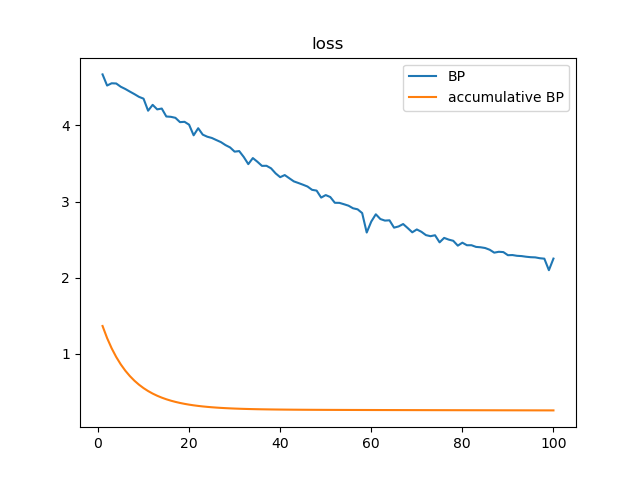
\includegraphics[scale=.9]{5.5/Figure_1.png}
\end{figure}
从图中可以看出,累积BP算法比标准BP算法收敛更快。

\end{document}
